\begin{frame}{Che cos'è l'Asset Allocation?}
	
    \begin{definition}
			L’\textbf{asset allocation} è il processo con il quale si decide in che modo distribuire le risorse fra diversi i possibili investimenti
    \end{definition}
	\begin{figure}
		\centering
		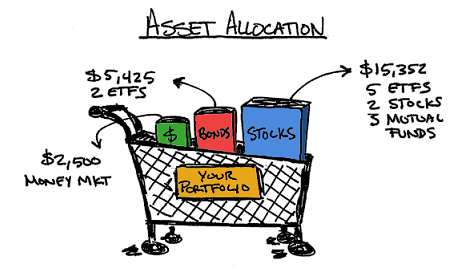
\includegraphics[width=.6\linewidth]{Images/AA}
	\end{figure}
\end{frame}


\begin{frame}{Raggiungibilità Stocastica: un esempio di applicazione}
	\begin{block}{Gestione del Traffico Aereo}
		\begin{figure}
			\centering
			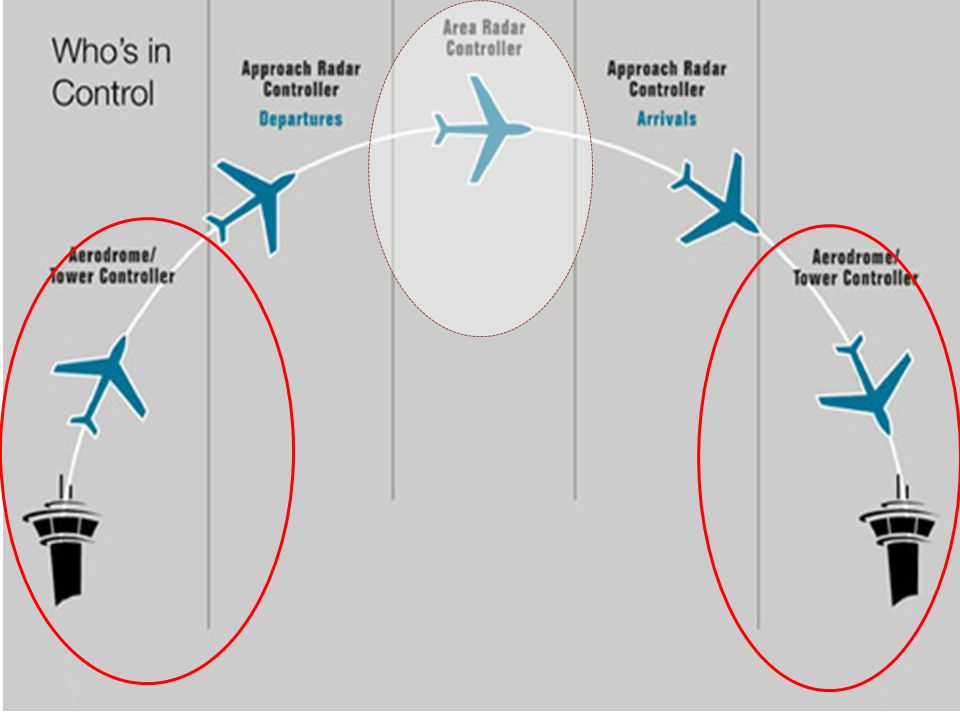
\includegraphics[width=0.7\linewidth]{Images/ATM}
		\end{figure}
	\end{block}
\end{frame}
\begin{frame}{Raggiungibilità Stocastica in Finanza}
	
		\begin{figure}
			\centering
			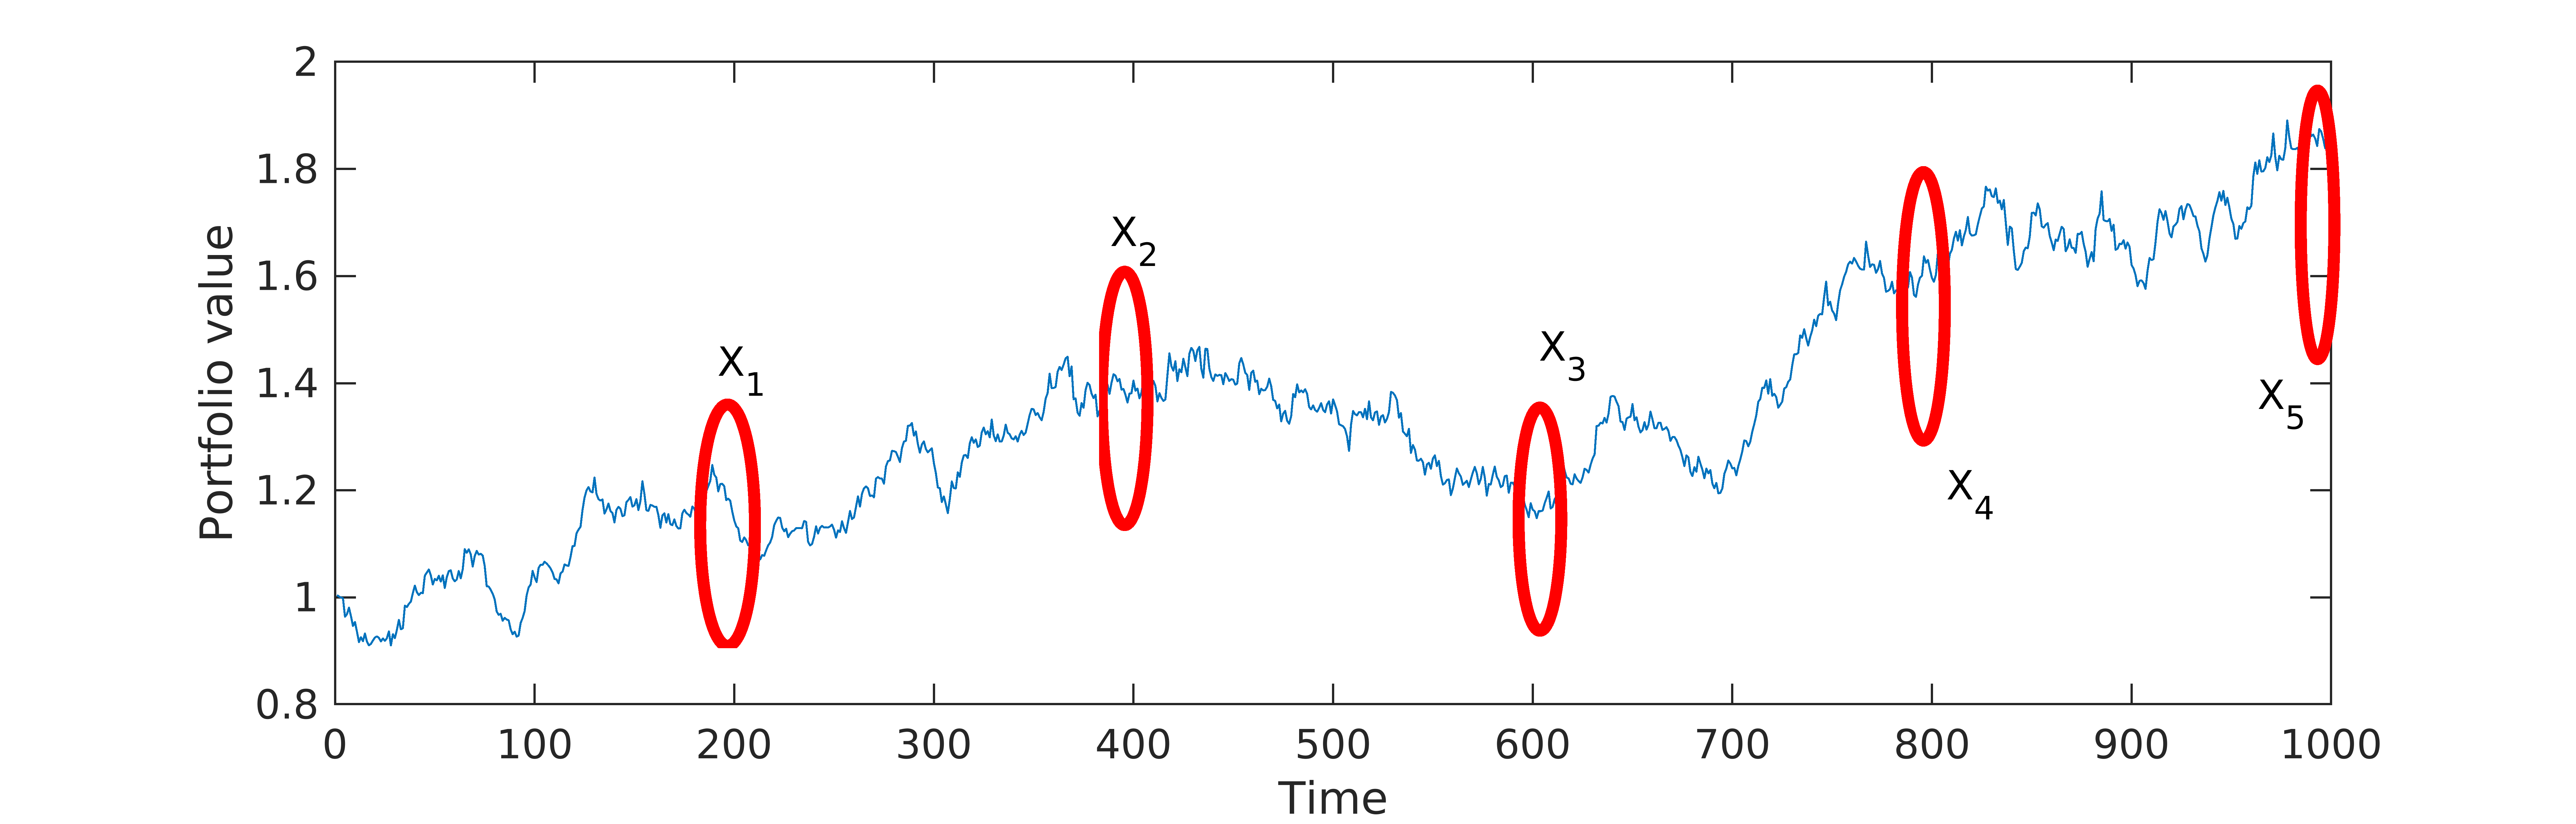
\includegraphics[width=1.1\linewidth]{Images/Reachability}
		\end{figure}

\end{frame}



